% Chapter 4 - Software Design Specification (rebuilt for the P2 Mid report)
\tikzset{
  box/.style={draw, rounded corners=2pt, minimum height=0.8cm, align=center, font=\footnotesize, fill=white},
  lay/.style={draw, rounded corners=3pt, fill=gray!8},
  arr/.style={-{Stealth[length=2mm]}, thick},
  ent/.style={draw, rectangle split, rectangle split parts=2, font=\scriptsize, align=left, fill=white, minimum width=3.4cm},
  cls/.style={draw, rectangle split, rectangle split parts=2, font=\scriptsize, align=left, fill=white, minimum width=3.0cm},
  phone/.style={draw, rounded corners=6pt, minimum width=3.6cm, minimum height=6.4cm, fill=white},
}

\chapter{Software Design Specification}

The Software Requirements Specification in Chapter 3 explains what Pakalorie must do.
This chapter explains how the system is designed to do it. It describes the architecture,
the twelve modules, the data stored by the system, the main components, the API, the
screens and the way the system is deployed. The design follows the layered approach
described by Bass et al.~\cite{sds_1} and uses UML notation~\cite{sq_diagrams} for the
diagrams. Implementation of this design is covered in Chapter~5, which also states which
modules are built and which are planned for the final milestone (Table~\ref{tab:status}).

\section{Introduction}
\subsection{Purpose}
The purpose of this Software Design Specification (SDS) is to give the development team,
the supervisor and the evaluators one clear description of the design of Pakalorie. Every
requirement in Table~3.1 is linked to a module in this chapter, so a reader can trace any
feature from requirement to design.

\subsection{Scope}
The SDS covers all twelve modules of Pakalorie: the React Native/Expo mobile app, the
FastAPI backend, the food recognition and depth models, the calorie engine, the databases,
and the external services (Firebase, the Claude and Gemini APIs, Google Fit and Apple
HealthKit). Source code is not part of this chapter; short code examples appear in
Chapter~5.

\subsection{Design Approach}
Three ideas guided the design.
\begin{itemize}[noitemsep]
  \item \textbf{Layered structure.} The mobile app, the API, the AI models and the data stores
        are separate layers. Each layer talks only to the layer next to it.
  \item \textbf{Modular structure.} Each of the twelve modules has one clear job and a small
        interface, so team members can work in parallel and test their own part.
  \item \textbf{API-first.} The mobile app calls a REST API for recognition and nutrition,
        which makes it easy to change models or add other clients later.
\end{itemize}

\section{Design Goals and Constraints}
\subsection{Design Goals}
\begin{itemize}[noitemsep]
  \item \textbf{Speed:} a result must reach the user within 3 seconds of image upload.
  \item \textbf{Simplicity:} the main task (capture, see result) must need no typing and no more
        than three interactions.
  \item \textbf{Accuracy:} recognition should reach at least 85\% top-1 accuracy on the
        Pakistani food dataset.
  \item \textbf{Privacy:} food photos are processed in memory and are not kept by the app.
  \item \textbf{Accessibility:} the app should work in English and Urdu, including
        right-to-left layout.
  \item \textbf{Maintainability:} modules must be independent enough to be changed or tested alone.
\end{itemize}

\subsection{Constraints}
\begin{itemize}[noitemsep]
  \item The app must run on mid-range phones (Android 8.0 and above, iOS 13.0 and above).
  \item Users may be on a normal 4G or WiFi connection, so images are compressed before upload.
  \item The project uses free or low-cost cloud services and open-source models.
  \item Recognition works on one image at a time. The live mode sends one camera frame at a
        time; it is not continuous video analysis.
  \item The system gives nutritional estimates only. It does not give medical advice.
\end{itemize}

\section{System Architecture}
Pakalorie uses a four-layer architecture, shown in Figure~\ref{fig:arch}. A fifth group,
external services, sits beside the layers.
\begin{itemize}[noitemsep]
  \item \textbf{Presentation Layer.} The React Native/Expo app. It shows the screens, uses the
        camera and gallery, compresses the image, and keeps a language setting for English and
        Urdu text.
  \item \textbf{Application Layer.} The FastAPI server. Routers handle recognition, food and
        nutrition data, calorie calculation and portion estimation. Every reply uses one
        envelope with a success flag, the data and an error message.
  \item \textbf{Intelligence Layer.} A YOLOv8 classifier names the dish, MiDaS estimates relative
        depth for a portion bucket, and the calorie engine retrieves nutrition rows and asks a
        language model to compose a grounded breakdown (retrieval-augmented generation, RAG).
  \item \textbf{Data Layer.} Firebase Authentication manages accounts. Cloud Firestore stores
        profiles, meals, water, activity and chat history. PostgreSQL stores the nutrition tables
        (USDA and local Pakistani data).
  \item \textbf{External Services.} The Anthropic Claude API writes the grounded calorie
        explanation and can also recognise a dish from a photo. The Google Gemini API is used by
        the chat coach and as an on-device fallback. Google Fit and Apple HealthKit are planned for
        health sync.
\end{itemize}

\begin{figure}[H]
\centering
\resizebox{\textwidth}{!}{%
\begin{tikzpicture}
  \draw[lay] (0,12) rectangle (14,9.6);
  \node[font=\footnotesize\bfseries, anchor=north west] at (0.15,11.92) {Presentation Layer (React Native / Expo)};
  \node[box, minimum width=3.1cm] at (2.0,10.45) {Screens (Login, Scan,\\Result, Home, Trends)};
  \node[box, minimum width=3.1cm] at (5.4,10.45) {Camera, Gallery,\\Image Compression};
  \node[box, minimum width=3.1cm] at (8.6,10.45) {Language Setting\\(English / Urdu)};
  \node[box, minimum width=3.1cm] at (11.9,10.45) {Compensation and\\Live Scan Logic};

  \draw[lay] (0,9.1) rectangle (14,6.7);
  \node[font=\footnotesize\bfseries, anchor=north west] at (0.15,9.02) {Application Layer (FastAPI, Python)};
  \node[box, minimum width=3.1cm] at (2.0,7.55) {Recognition\\Router};
  \node[box, minimum width=3.1cm] at (5.4,7.55) {Foods\\Router};
  \node[box, minimum width=3.1cm] at (8.6,7.55) {Calories\\Router};
  \node[box, minimum width=3.1cm] at (11.9,7.55) {Portion (Depth)\\Router};

  \draw[lay] (0,6.2) rectangle (14,3.8);
  \node[font=\footnotesize\bfseries, anchor=north west] at (0.15,6.12) {Intelligence Layer};
  \node[box, minimum width=3.1cm] at (2.0,4.65) {YOLOv8\\Classifier};
  \node[box, minimum width=3.1cm] at (5.4,4.65) {MiDaS\\Depth (ONNX)};
  \node[box, minimum width=3.1cm] at (8.6,4.65) {Calorie Engine\\+ Retriever (RAG)};
  \node[box, minimum width=3.1cm] at (11.9,4.65) {Claude\\Client};

  \draw[lay] (0,3.3) rectangle (14,0.9);
  \node[font=\footnotesize\bfseries, anchor=north west] at (0.15,3.22) {Data Layer};
  \node[box, minimum width=3.9cm] at (2.4,1.75) {Firebase\\Authentication};
  \node[box, minimum width=3.9cm] at (7.0,1.75) {Cloud Firestore\\(users, meals, chat)};
  \node[box, minimum width=3.9cm] at (11.6,1.75) {PostgreSQL\\(USDA + local data)};

  \draw[lay] (0,0.4) rectangle (14,-2.0);
  \node[font=\footnotesize\bfseries, anchor=north west] at (0.15,0.32) {External Services};
  \node[box, minimum width=5.0cm] at (4.0,-1.15) {Anthropic Claude API\\Google Gemini API};
  \node[box, minimum width=5.0cm] at (10.2,-1.15) {Google Fit / Apple HealthKit\\(planned)};

  \draw[arr] (7,9.6) -- node[right, font=\scriptsize]{HTTPS (REST)} (7,9.1);
  \draw[arr] (7,6.7) -- node[right, font=\scriptsize]{model calls} (7,6.2);
  \draw[arr] (7,3.8) -- node[right, font=\scriptsize]{queries and storage} (7,3.3);
  \draw[arr] (7,0.9) -- node[right, font=\scriptsize]{external APIs} (7,0.4);
\end{tikzpicture}}
\caption{Layered Architecture of Pakalorie}
\label{fig:arch}
\end{figure}

\paragraph{Main data flow.} When a user scans a meal, the app compresses the photo and sends it
to the recognition router. The server names the dish with the chosen engine (the trained YOLOv8
model or the Claude vision model). The app then calls the calorie router, which reads the matching
nutrition rows from PostgreSQL, applies the portion and any modifiers, and returns the calories and
macronutrients with a short explanation and the source rows. If the user saves the meal, the app
writes it to Firestore. Portion estimation with MiDaS is a separate endpoint.

\section{Module Design}
Table~\ref{tab:modules} lists the twelve modules, the layer they mainly belong to, their main
technology, and the functional requirements (FR) from Chapter 3 that they satisfy. Together the
modules cover FR1 to FR32.

\begin{table}[H]
\centering
\caption{Module Summary and Requirement Mapping}
\label{tab:modules}
\small
\begin{tabularx}{\textwidth}{|c|>{\raggedright\arraybackslash}X|l|>{\raggedright\arraybackslash}X|l|}
\hline
\textbf{No.} & \textbf{Module} & \textbf{Layer} & \textbf{Main Technology} & \textbf{FRs} \\ \hline
1 & Authentication and User Management & Presentation, Data & Firebase Auth, Firestore & FR1--FR5 \\ \hline
2 & Core Mobile UI (Capture and Results) & Presentation & React Native, Expo & FR6--FR10 \\ \hline
3 & Food Recognition & Intelligence & YOLOv8 classifier (Ultralytics) & FR11--FR14 \\ \hline
4 & Food Database API & Application, Data & FastAPI, PostgreSQL & FR15, FR16 \\ \hline
5 & Volume and Depth Estimation & Intelligence & MiDaS (ONNX) & FR17, FR18 \\ \hline
6 & Calorie Calculation Engine with RAG & Intelligence & Python, retriever, Claude & FR19 \\ \hline
7 & Model Optimisation and Quantisation & Intelligence & ONNX Runtime INT8 & FR21 \\ \hline
8 & Data Visualisation and Calorie Compensation & Presentation & SVG charts, TypeScript & FR20, FR22, FR23 \\ \hline
9 & Real-Time Inference Pipeline & Application & Camera frames, FastAPI & FR24 \\ \hline
10 & Urdu Localisation & Presentation & i18n, RTL layout & FR25, FR26 \\ \hline
11 & Health Data Sync & Presentation, External & Google Fit, HealthKit & FR27--FR29 \\ \hline
12 & AI Chat Coach & Application, External & Gemini API, RAG & FR30--FR32 \\ \hline
\end{tabularx}
\end{table}

\subsection{Module 1: Authentication and User Management}
\textbf{Purpose:} register users, sign them in and protect their data. \textbf{Inputs:} email and
password, or a Google account. \textbf{Processing:} Firebase Authentication checks the credentials
and returns an ID token. The app keeps the session and loads the profile document from Firestore.
\textbf{Outputs:} a signed-in session and a profile document (name, weight, height, goal, daily
calorie target) in Firestore.

\subsection{Module 2: Core Mobile UI (Capture and Results)}
\textbf{Purpose:} give the user the shortest path from photo to result. \textbf{Inputs:} a camera
photo or a gallery image. \textbf{Processing:} the image is compressed and sent to the server. A
loading state is shown while waiting. \textbf{Outputs:} a result card with the dish name, a
confidence score, the calories, protein, carbohydrates and fat, a source label showing that the
numbers come from the database, and a disclaimer. The user can choose a meal type and save the
meal to history.

\subsection{Module 3: Food Recognition}
\textbf{Purpose:} name the food in a photo. \textbf{Inputs:} the decoded image. \textbf{Processing:}
a YOLOv8n classification model trained on 217 Pakistani and international dish classes returns the
most likely labels with confidence scores. The user can choose in Settings between the Claude vision
engine and the trained YOLOv8 engine. \textbf{Outputs:} the best label, its confidence and the next
most likely labels as alternatives. The original design used object detection with bounding boxes to
find several items in one photo; the built model is a classifier, so it names one dish per image.

\subsection{Module 4: Food Database API}
\textbf{Purpose:} serve nutrition data. \textbf{Inputs:} a food identifier or a search text.
\textbf{Processing:} the API queries PostgreSQL, which holds 160 foods (30 curated Pakistani dishes
and 130 USDA items) with English and Urdu names, aliases, labelled portions, nutrition facts and
additive modifiers such as extra oil. \textbf{Outputs:} calories, protein, carbohydrates and fat for
the requested portion, as JSON.

\subsection{Module 5: Volume and Depth Estimation}
\textbf{Purpose:} adjust calories to the portion size. \textbf{Inputs:} the image. \textbf{Processing:}
MiDaS creates a relative depth map from the single image. A simple rule combines depth and plate
area into a portion bucket (small, medium or large) with a multiplier. No reference object is needed.
\textbf{Outputs:} a portion bucket and multiplier. The result is relative, not a measurement in grams.

\subsection{Module 6: Calorie Calculation Engine with RAG}
\textbf{Purpose:} turn a recognised dish and a portion into nutrition totals. \textbf{Inputs:} the dish,
portion, servings and modifiers. \textbf{Processing:} the engine retrieves the matching rows from the
database, scales them for the portion and modifiers, and asks the Claude model to compose the answer
using only those rows. If the model is unavailable, a local calculation from the same rows is returned.
\textbf{Outputs:} calories and macros, a short explanation and the source rows.

\subsection{Module 7: Model Optimisation and Quantisation}
\textbf{Purpose:} make the recognition model small enough for phones and a modest server.
\textbf{Inputs:} the trained YOLOv8n classification model in ONNX format (217 classes,
$224\times224$ input). \textbf{Processing:} the model is quantised to 8-bit integers in two ways:
dynamic quantisation, which converts only the weights, and static quantisation, which also converts
the activations using 200 calibration images. Each version is compared with the original for file size,
CPU latency and accuracy on the same held-out images. \textbf{Outputs:} a comparison table
(Table~\ref{tab:quant}) and the recommended model file.

\subsection{Module 8: Data Visualisation and Calorie Compensation}
\textbf{Purpose:} help the user see trends and keep to the daily goal after a heavy or light day.
\textbf{Inputs:} saved meals, activities logged by the user, and the daily calorie goal.
\textbf{Processing:} meals are grouped by day. The module looks at the last three days on which the user
logged meals. The surplus (calories eaten minus the goal plus the calories burned that day) is added up
and divided by three, so each day's surplus is repaid over three days. The change to today's goal is
limited to 15\% of the base goal and never takes the goal below a safe minimum of 1200~kcal (or below the
user's own goal, if that is already lower). Calories burned by logged activity are added to today's goal.
\textbf{Outputs:} an adjusted daily goal with a one-line explanation, a disclaimer that the numbers are
estimates and not medical advice, and charts of calories, macronutrient share, weight and water intake.

\subsection{Module 9: Real-Time Inference Pipeline}
\textbf{Purpose:} give the user a result while the camera is pointed at the food, without pressing the
shutter. \textbf{Processing:} in live mode the app captures a small, low-quality camera frame, sends it
to the recognition service with the YOLOv8 engine, and shows the best guess with its confidence. Only one
frame is in flight at a time; the next frame is captured as soon as the reply arrives, so the server
latency sets the frame rate. Guesses below 35\% confidence are labelled ``low confidence''. The live mode
uses only the YOLOv8 model, so it does not call any paid language-model service. \textbf{Outputs:} a live
label, the confidence, the round-trip time and the frames per second. In this version the pipeline is
streamed from the phone to the server; running the quantised model on the phone itself is future work.

\subsection{Module 10: Urdu Localisation}
\textbf{Purpose:} make the app usable for people who prefer Urdu. \textbf{Processing:} screen text is
kept in translation files for English and Urdu. When Urdu is chosen the layout switches to right-to-left.
Food names come from the database, which stores both an English and an Urdu name.
\textbf{Outputs:} a translated interface that can be changed without restarting the app.
This module is planned for the final milestone.

\subsection{Module 11: Health Data Sync}
\textbf{Purpose:} join nutrition and activity data in one place. \textbf{Processing:} with the user's
permission, saved meals are written to Google Fit (Android) or Apple HealthKit (iOS), and activity data
such as steps is read back. \textbf{Outputs:} a unified health dashboard that shows intake next to
activity. This module is planned for the final milestone.

\subsection{Module 12: AI Chat Coach}
\textbf{Purpose:} answer food and health questions in simple language. \textbf{Inputs:} the user's
message, profile and today's totals. \textbf{Processing:} the app builds a prompt from fixed safety rules,
the user's remaining calories, macros and goal, and the question, and sends it to the Gemini API.
\textbf{Outputs:} a reply in the chat screen. The design calls for the server to retrieve nutrition facts
and keep the API key; the built version calls the model from the app (Section~\ref{sec:coach}).

\section{Data Design}
Pakalorie uses two databases. Firebase Firestore stores user-specific data that changes often and must
sync across devices. PostgreSQL stores the fixed nutrition reference data, which is relational and needs
fast lookups and search~\cite{user_table}.

\subsection{PostgreSQL Schema}
Figure~\ref{fig:erd} shows the nutrition database. \texttt{foods} holds one row per food with its English
and Urdu name, category and source. \texttt{food\_aliases} stores other names and spellings, including
Urdu, so search works in both languages. \texttt{portion\_sizes} lists the labelled portions of a food.
\texttt{nutrition\_facts} holds the calories and macronutrients for each portion, and
\texttt{modifier\_constants} holds additive changes such as extra oil.

\begin{figure}[H]
\centering
\begin{tikzpicture}[node distance=1.2cm]
  \node[ent] (foods) {\textbf{foods}\nodepart{second}PK id\\source, source\_id\\name\_en, name\_ur\\slug, category\\base\_unit, description};
  \node[ent, right=1.6cm of foods, yshift=1.4cm] (alias) {\textbf{food\_aliases}\nodepart{second}PK id\\FK food\_id\\alias, language};
  \node[ent, right=1.6cm of foods, yshift=-0.9cm] (port) {\textbf{portion\_sizes}\nodepart{second}PK id\\FK food\_id\\label, weight\_g\\is\_default};
  \node[ent, below=0.9cm of port] (nut) {\textbf{nutrition\_facts}\nodepart{second}PK id\\FK food\_id, FK portion\_id\\calories\_kcal\\protein\_g, carbs\_g, fat\_g\\fiber\_g (optional)};
  \node[ent, below=0.9cm of foods] (mod) {\textbf{modifier\_constants}\nodepart{second}PK id\\FK food\_id\\name, kcal\_delta\\description};
  \draw[arr] (foods) -- node[above, font=\scriptsize]{1 : N} (alias);
  \draw[arr] (foods) -- node[above, font=\scriptsize]{1 : N} (port);
  \draw[arr] (port) -- node[right, font=\scriptsize]{1 : N} (nut);
  \draw[arr] (foods) -- node[left, font=\scriptsize]{1 : N} (mod);
\end{tikzpicture}
\caption{Entity Relationship Diagram of the Nutrition Database}
\label{fig:erd}
\end{figure}

\subsection{Firestore Structure}
Table~\ref{tab:firestore} describes the Firestore collections. All data sits under the user's own ID, and
security rules allow a user to read and write only their own documents. Each query filters on a single
field, so no composite indexes are needed.

\begin{table}[H]
\centering
\caption{Firestore Data Dictionary}
\label{tab:firestore}
\small
\begin{tabularx}{\textwidth}{|>{\ttfamily\scriptsize\raggedright\arraybackslash}p{5.3cm}|>{\raggedright\arraybackslash}X|>{\raggedright\arraybackslash}p{3.0cm}|}
\hline
\textbf{Path} & \textbf{Main Fields} & \textbf{Purpose} \\ \hline
users/\{uid\} & display\_name, gender, current\_weight\_kg, height\_cm, goal\_type, activity\_level, daily\_target\_kcal, onboarding\_complete & Profile, goals and settings \\ \hline
users/\{uid\}/food\_logs & name, calories, protein, carbs, fat, meal\_type, created\_at & One saved meal \\ \hline
users/\{uid\}/activity\_logs & log\_date, activity, minutes, kcal, created\_at & Logged activity for compensation \\ \hline
users/\{uid\}/hydration/\{day\} & log\_date, count & Glasses of water per day \\ \hline
users/\{uid\}/weight\_logs & weight\_kg, logged\_at & Weight history \\ \hline
users/\{uid\}/favorites & food name and nutrition values & Saved favourite foods \\ \hline
users/\{uid\}/chat\_sessions & messages, timestamps & AI coach conversation \\ \hline
\end{tabularx}
\end{table}

\subsection{Data Handling Rules}
\begin{itemize}[noitemsep]
  \item Food photos are not stored by the app. Only the result (name and nutrition values) is saved to the
        meal history.
  \item Nutrition values in PostgreSQL are read-only for normal users.
  \item The Firestore rules allow a signed-in user to read and write only their own tree.
\end{itemize}

\section{Component Design}
Figure~\ref{fig:class} shows the main components. Each one matches a module, which keeps the code close
to the design.
\begin{itemize}[noitemsep]
  \item \texttt{AuthContext} signs users in and keeps the profile (Module 1).
  \item \texttt{YoloRecognizer} loads the ONNX classifier once and returns the best labels (Module 3).
  \item \texttt{DepthEstimator} runs MiDaS and returns a portion bucket (Module 5).
  \item \texttt{CalorieEngine} reads rows through the retriever, scales them, and asks \texttt{ClaudeClient}
        to write the grounded answer (Module 6).
  \item \texttt{compensation} computes the adjusted daily goal and the burn estimate (Module 8).
  \item \texttt{useLiveRecognition} runs the live loop on the phone (Module 9).
\end{itemize}
The design uses a few common patterns~\cite{interface_1}. The food service is a repository, so the rest
of the code does not depend on SQL. The calorie engine gives the router a single call for the whole
calculation. Each model is loaded only once, when it is first needed.

\begin{figure}[H]
\centering
\resizebox{\textwidth}{!}{%
\begin{tikzpicture}[node distance=0.9cm]
  \node[cls] (auth) {\textbf{AuthContext}\nodepart{second}signIn, signUp\\updateProfile\\profile};
  \node[cls, right=1.1cm of auth] (live) {\textbf{useLiveRecognition}\nodepart{second}capture frame\\call /recognize\\fps, latency};
  \node[cls, right=1.1cm of live] (yolo) {\textbf{YoloRecognizer}\nodepart{second}recognize(image)\\top-k labels\\confidence};
  \node[cls, right=1.1cm of yolo] (depth) {\textbf{DepthEstimator}\nodepart{second}estimate(image)\\portion bucket};
  \node[cls, below=1.3cm of yolo] (eng) {\textbf{CalorieEngine}\nodepart{second}breakdown(dish, portion)\\fallback if no model};
  \node[cls, left=1.1cm of eng] (food) {\textbf{FoodService}\nodepart{second}search(q)\\getFood(id)\\nutrition(portion)};
  \node[cls, right=1.1cm of eng] (claude) {\textbf{ClaudeClient}\nodepart{second}generate\_json(prompt)};
  \node[cls, below=1.3cm of food] (comp) {\textbf{compensation}\nodepart{second}computeCompensation\\estimateBurn};
  \draw[arr] (live) -- node[above, font=\scriptsize]{calls} (yolo);
  \draw[arr] (eng) -- node[above, font=\scriptsize]{reads} (food);
  \draw[arr] (eng) -- node[above, font=\scriptsize]{uses} (claude);
  \draw[arr] (eng.north east) -- node[above, font=\scriptsize, sloped]{uses} (depth.south west);
\end{tikzpicture}}
\caption{Main Components}
\label{fig:class}
\end{figure}

\section{API Design}
All endpoints are REST endpoints and use JSON. Every reply uses one envelope with the fields
\texttt{success}, \texttt{data} and \texttt{error}. The endpoints are described in Table~\ref{tab:api}.
The current server does not check Firebase tokens; it is protected by HTTPS only, and token checking is
planned (Section~\ref{sec:security}).

\begin{table}[H]
\centering
\caption{Main API Endpoints}
\label{tab:api}
\small
\begin{tabularx}{\textwidth}{|>{\ttfamily\raggedright\arraybackslash}p{4.9cm}|>{\raggedright\arraybackslash}p{3.0cm}|>{\raggedright\arraybackslash}X|}
\hline
\textbf{Method and Path} & \textbf{Input} & \textbf{Output and Purpose} \\ \hline
GET /healthz & none & Server health check \\ \hline
POST /recognize & image file, engine & Best dish label, confidence and alternatives (FR11, FR15) \\ \hline
GET /foods/search & q, limit & Fuzzy search in English, Roman Urdu or Urdu \\ \hline
GET /foods/\{id\} & food id & Food with portions and modifiers (FR16) \\ \hline
POST /foods/\{id\}/nutrition & portion, modifiers & Adjusted nutrition values \\ \hline
POST /calories & dish, portion, servings & Grounded calories and macros, explanation and source rows (FR19) \\ \hline
POST /portion & image & Relative depth portion bucket (FR17, FR18) \\ \hline
\end{tabularx}
\end{table}

Errors use standard HTTP codes, for example 422 for invalid input and 503 when a model is not ready. Every
error reply has a short message that the app can show.

\section{User Interface Design}
\subsection{Design Principles}
The interface follows basic usability rules~\cite{custom_technique_1(0),user_interface}. There is one main action
on the home screen (scan). Calories are shown first and largest, because test users asked for this in
Chapter 3. Text is short and written in plain words. Buttons are large enough for one-handed use.

\subsection{Screen Flow}
Figure~\ref{fig:flow} shows how screens connect. A new user sees the welcome screen, sign-up and
onboarding, and then reaches the home screen. A bottom tab bar links the main areas.

\begin{figure}[H]
\centering
\resizebox{\textwidth}{!}{%
\begin{tikzpicture}[node distance=0.6cm]
  \node[box] (w) {Welcome};
  \node[box, right=of w] (s) {Sign up /\\Login};
  \node[box, right=of s] (o) {Onboarding\\(goal, body, target)};
  \node[box, right=of o] (h) {Home\\(budget card)};
  \node[box, above=0.9cm of h, minimum width=7cm] (tab) {Tabs: Home, Ustad (chat), Search, Profile, Trends,\\Calendar log, Water, Achievements};
  \node[box, below=1.2cm of h] (sc) {Scan\\(camera, gallery, Live)};
  \node[box, left=of sc] (r) {Result\\(grounded calories)};
  \node[box, left=of r] (log) {Save meal\\(Firestore)};
  \draw[arr] (w)--(s); \draw[arr] (s)--(o); \draw[arr] (o)--(h);
  \draw[arr] (h)--(sc); \draw[arr] (sc)--(r); \draw[arr] (r)--(log);
  \draw[arr] (tab)--(h);
\end{tikzpicture}}
\caption{Screen Navigation Flow}
\label{fig:flow}
\end{figure}

\subsection{Wireframes}
Figure~\ref{fig:wire} shows three core screens: login, home with the budget card, and the result. They
follow the low-fidelity wireframes reviewed by test users in Chapter 3.

\begin{figure}[H]
\centering
\resizebox{\textwidth}{!}{%
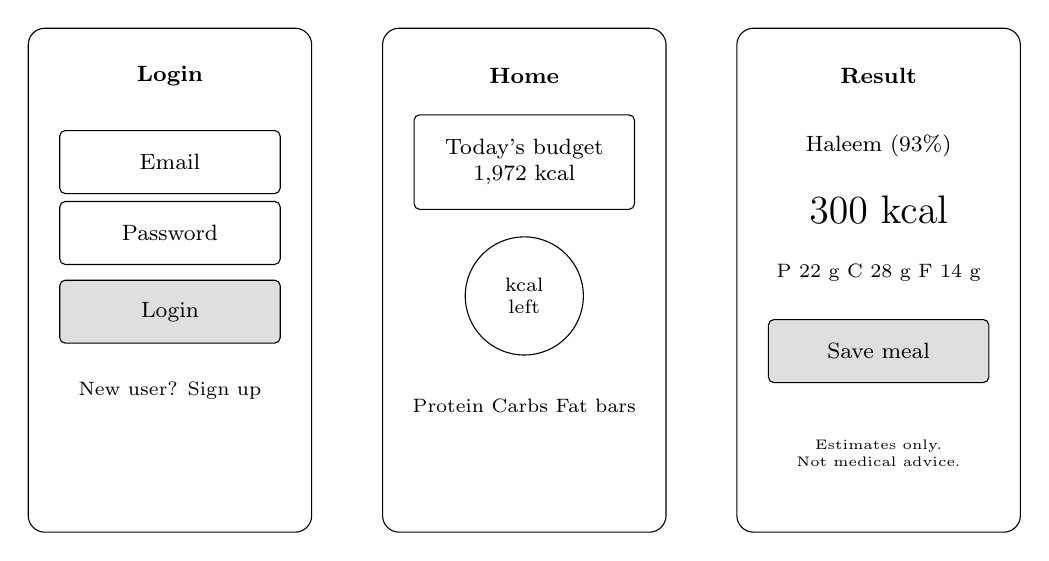
\begin{tikzpicture}
  \node[phone] at (0,0) {};
  \node[font=\footnotesize\bfseries] at (0,2.6) {Login};
  \node[box, minimum width=2.8cm] at (0,1.5) {Email};
  \node[box, minimum width=2.8cm] at (0,0.6) {Password};
  \node[box, minimum width=2.8cm, fill=gray!25] at (0,-0.4) {Login};
  \node[font=\scriptsize] at (0,-1.4) {New user? Sign up};
  \node[phone] at (4.5,0) {};
  \node[font=\footnotesize\bfseries] at (4.5,2.6) {Home};
  \node[box, minimum width=2.8cm, minimum height=1.2cm] at (4.5,1.5) {Today's budget\\1,972 kcal};
  \node[draw, circle, minimum size=1.5cm, font=\scriptsize, align=center] at (4.5,-0.2) {kcal\\left};
  \node[font=\scriptsize] at (4.5,-1.6) {Protein  Carbs  Fat bars};
  \node[phone] at (9,0) {};
  \node[font=\footnotesize\bfseries] at (9,2.6) {Result};
  \node[font=\footnotesize] at (9,1.7) {Haleem  (93\%)};
  \node[font=\Large] at (9,0.9) {300 kcal};
  \node[font=\scriptsize] at (9,0.1) {P 22 g   C 28 g   F 14 g};
  \node[box, minimum width=2.8cm, fill=gray!25] at (9,-0.9) {Save meal};
  \node[font=\tiny, text width=3cm, align=center] at (9,-2.2) {Estimates only.\\Not medical advice.};
\end{tikzpicture}}
\caption{Wireframes of the Login, Home and Result Screens}
\label{fig:wire}
\end{figure}

\subsection{Screen Descriptions}
Table~\ref{tab:screens} lists the main screens and what each one shows.

\begin{table}[H]
\centering
\caption{Main Screens}
\label{tab:screens}
\small
\begin{tabularx}{\textwidth}{|>{\raggedright\arraybackslash}p{3.6cm}|>{\raggedright\arraybackslash}X|}
\hline
\textbf{Screen} & \textbf{Content} \\ \hline
Sign up / Login & Email and password fields, error messages \\ \hline
Onboarding & Goal, age, gender, height and weight, activity level and the calculated daily target \\ \hline
Home & Calories left ring, eaten and target, macro bars, today's budget card with activity log, water counter \\ \hline
Scan & Camera preview, capture button, gallery button, Live mode toggle \\ \hline
Result & Dish name and confidence, calories and macros, source label, meal type, save button, disclaimer \\ \hline
Search & Food search and quick logging \\ \hline
Trends & Calorie, macro split, weight and water charts for 7, 30 or 90 days \\ \hline
Ustad (chat) & Chat window with text input \\ \hline
Profile and Settings & Personal data, calorie target, recognition engine, sign out \\ \hline
\end{tabularx}
\end{table}

\section{Security and Privacy Design}\label{sec:security}
\begin{itemize}[noitemsep]
  \item \textbf{Authentication:} Firebase Authentication with email and password. Passwords are never
        handled by Pakalorie's own server. Google sign-in is wired in the code but needs a development
        build to test.
  \item \textbf{Authorisation:} Firestore rules restrict each user to their own documents. Verifying the
        Firebase token on each API request is planned but not yet built.
  \item \textbf{Transport:} all traffic between app and server uses HTTPS/TLS.
  \item \textbf{Secrets:} the Claude API key and database passwords are kept in server environment
        variables, never in the app. The Gemini key used by the chat coach and the offline fallback is
        currently read from the app configuration; moving it to the server is future work.
  \item \textbf{Images:} intended to be processed in memory and not stored.
  \item \textbf{Medical safety:} a disclaimer on the result screen and in the budget card says the app
        gives estimates, not medical advice.
\end{itemize}

\section{Deployment Design}
Figure~\ref{fig:deploy} shows deployment. The backend runs as Docker containers on one server: the FastAPI
container and a PostgreSQL container on a private Docker network. Caddy is the only service open to the
internet; it terminates HTTPS and forwards requests to the API. Firebase and the Claude API are managed cloud
services. Docker gives the same environment on every machine and makes the move from laptop to server simple.

\begin{figure}[H]
\centering
\resizebox{\textwidth}{!}{%
\begin{tikzpicture}
  \node[box, minimum width=3.4cm] (app) at (0,0) {Pakalorie App\\(React Native / Expo)};
  \node[lay, minimum width=7.6cm, minimum height=4.0cm] (srv) at (7.0,-0.2) {};
  \node[font=\footnotesize\bfseries, anchor=north west] at (srv.north west) {Server (Docker host)};
  \node[box] (caddy) at (4.7,0.1) {Caddy\\(HTTPS)};
  \node[box] (api) at (7.5,0.1) {FastAPI\\(YOLO, MiDaS,\\Calorie Engine)};
  \node[box] (pg) at (7.5,-1.45) {PostgreSQL\\(nutrition data)};
  \node[box] (fb) at (13.2,3.0) {Firebase\\(Auth + Firestore)};
  \node[box] (cl) at (13.2,-1.2) {Anthropic\\Claude API};
  \draw[arr] (app) -- node[above, pos=0.3, font=\scriptsize]{HTTPS} (caddy);
  \draw[arr] (caddy) -- (api);
  \draw[arr] (api) -- node[left, font=\scriptsize]{SQL} (pg);
  \draw[arr] (api.east) to[out=0,in=180] (cl.west);
  \draw[arr] (app.north) |- node[above, pos=0.75, font=\scriptsize]{Firebase SDK} (fb.west);
\end{tikzpicture}}
\caption{Deployment Diagram}
\label{fig:deploy}
\end{figure}

\needspace{12\baselineskip}
\section{Design Decisions and Justification}
\begin{table}[H]
\centering
\caption{Key Design Decisions}
\label{tab:decisions}
\small
\begin{tabularx}{\textwidth}{|>{\raggedright\arraybackslash}p{3.2cm}|>{\raggedright\arraybackslash}p{3.6cm}|>{\raggedright\arraybackslash}X|}
\hline
\textbf{Decision} & \textbf{Choice} & \textbf{Reason} \\ \hline
Recognition model & YOLOv8 classification, with a Claude vision option & Trains on folder-per-dish images without box labels; runs fast on modest hardware~\cite{yolo_ult}. The Claude option gives a strong fallback \\ \hline
Portion size & MiDaS depth from one image & Works without a reference object or special hardware~\cite{midas} \\ \hline
Mobile framework & React Native with Expo & One code base for Android and iOS~\cite{expo} \\ \hline
Backend & FastAPI (Python) & Same language as the models; async support; automatic API docs~\cite{fastapi} \\ \hline
User data & Firestore & Real-time sync, built-in security rules, works with Firebase Auth~\cite{firebase} \\ \hline
Nutrition data & PostgreSQL & Structured data, fast search, easy to extend with new foods \\ \hline
Calorie answers & Retrieval from the database, then Claude & Grounds answers in real nutrition rows and reduces invented numbers~\cite{rag,anthropic} \\ \hline
Deployment & Docker with Caddy & Repeatable setup and simple HTTPS~\cite{docker,caddy} \\ \hline
\end{tabularx}
\end{table}
